%% zusammenf.tex
%% $Id: zusammenf.tex 4 2005-10-10 20:51:21Z bless $
%%

\chapter{Future Work}
\label{ch:FutureWork}
%% ==============================
%
The Accessible EPUB editor is in a functional state where accessible EPUBs of the both new document standards, CSS and JavaScript can be created and edited. However, there is still much to be done.

The JavaScript document standard supports multiple HTML files as content documents. If the reading system supports local or session storage, it remembers which display style is to be displayed across several HTML files. This is actually the case with JavaScript standard in its current state as the first page with version switching mechanism is on a different page from the actual content. Accessible EPUB does not yet support multiple content pages. One issue mentioned in chapter \ref{ch:AccessibleEPUB Editor} is there are issues with long documents. The preview browser automatically scrolls to the top as soon as the user writes something in the editor. If Accessible EPUB allows the user to add another content page, this problem can be avoided. Furthermore, the user can create documents with several sections and these can be managed individually. This does not work with the CSS standard as CSS changes are local to a HTML file and do not persist across multiple of them.

Future development will focus on usability and simplified import of other document standards. Allowing users to import files of different formats will allow an easier transition to Accessible EPUB. The features will be implemented for two formats at first: text documents and HTML files. Importing text documents is quite simple as the file just has to be read and the contents have to be inserting into the editor. Importing HTML files is a bit more complicated. Instead of inserting into the editor, the back end web browser of the editor must be inserted to. Images and equations will not be in the form of the accessible EPUB document standard, so they have to be converted into the correct form. The program will present the user with a process to examine every image and equation and insert alternative text when necessary. Other formats can be imported with the tool pandoc converting them. It is already a part of Accessible EPUB so it does not require any additional programs.

Another feature advanced users may want is a source code editor. As mentioned in chapter \ref{ch:AccessibleEPUB Editor} a code viewer is already available, but it currently displays the entire file with the inner workings. It is also disabled as there were several issues with it. If a code editor is included, the user should not be able to see the inner workings of the document standard, since editing those might break the EPUB file and make it unreadable. 

\begin{comment}
\begin{figure}
	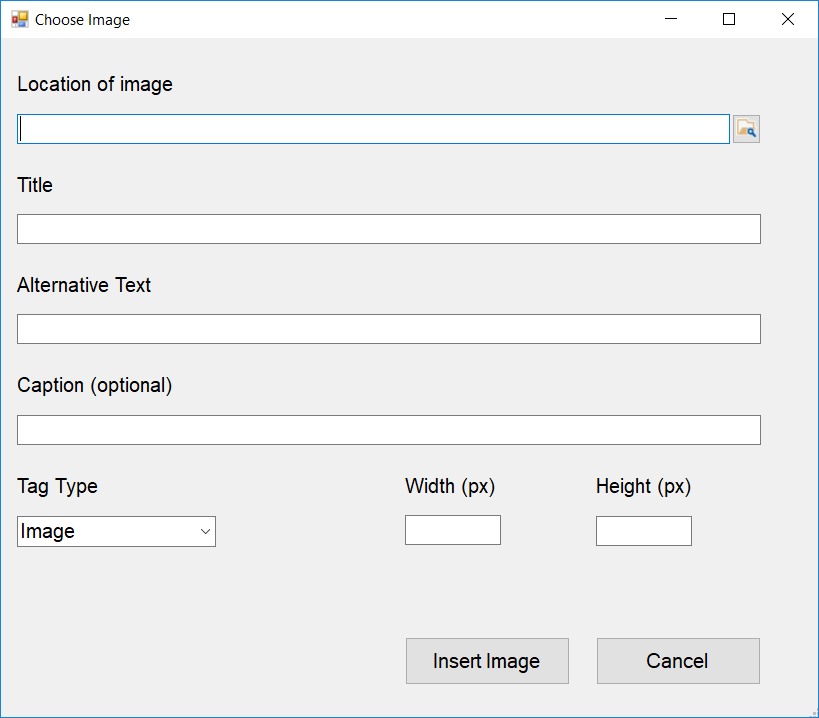
\includegraphics[width=\linewidth]{figures/imageDialogBox.png}	
	\caption{Insert image window of Accessible EPUB}
	\label{fig:imageDialogBox1}
\end{figure}
\end{comment}

To improve accessibility for visually impaired users, it should be possible to add an alternative image which can be a high contrast version of the original image. In addition to the one image document creators have to add, there will be an option to another one. This image will only be shown in the visually impaired display style. If no secondary image was chosen, the regular image will be displayed instead.

Training material has to be prepared so that users can get to know the EPUB standard and Accessible EPUB, like workshops which will users to test the standard and program. There will also be step-by-step tutorials to guide people through the document creation process and how to use all tools in the program.


\begin{comment}
There is still some room for improvement in the compatibility of the EPUB standard, so that it will also be possible to use the documents better with "older" EPUB readers. 
The JavaScript document standard supports multiple HTML files as content documents. If the reader system supports local or session storage, it remembers which version is to be displayed across several HTML files. Accessible EPUB does not yet support this. Adding this feature would allow users to create longer documents and manage individual sections.

Future development will focus on usability and simplified import of other document standards. Currently, users can already import text and HTML documents with certain restrictions so that they can keep their work in these formats. The tool PANDOC can serve as a basis for many formats.
Furthermore, images and formulas will not yet be in the format specified by the document standard during an import, so a wizard will be added that works through each image and formula and allows the user to enter alternative texts.  

Another feature advanced users may want is a source code editor. A code viewer is already available, but currently displays the entire file with the inner workings. The user should not be able to see it, since the processing increases the error possibilities in the document.

We are also considering whether we will start developing suitable readers for various end devices.
\end{comment}

\chapter{Conclusion}
\label{ch:Conclusion}

A short introduction is given where the motivation of this project and a short overview of the file format EPUB is presented. An EPUB document standard has been developed to allow visually impaired, blind and normal-sighted users to use the same document while meeting their respective accessibility requirements. There are two different versions of it, one using JavaScript and the other using CSS. Both versions of the document standard were tested on several reading systems. Only very few of the reading systems were able to show MathML equations and even fewer were able to display the document standards properly. 

EPUB 3 is not widely supported by reading systems. The switching mechanism only worked on four out of fourteen. MathML rendered on nine of them, and many reading systems were chosen because they supported it. Developers still have a lot of work to do for EPUB 3 to have support in their reading systems.

An editor called "Accessible EPUB" was created so that users without programming knowledge can create accessible documents. It allows the user to write text much like in an word processor and insert mathematical equations, images and tables. The document standard uses EPUB 3, which is not yet fully supported by most EPUB reading systems. It is planned to add features to improve the usability of Accessible EPUB, such as importing files of different formats and further tools for accessibility.
